We investigated three versions of the AWP design described in the last section of the previous chapter. The first type we present is based on 3D printed \ce{Al2O3}, the second type is produced using ordinary 3D printed polymers and the third type consists of SLE fused silica glass waveplates as described in the previous chapter. The results are obtained through the minimization of the two objective functions defined in the previous chapter.

% This AWP type differs from the other two in the sense that the phase shift is not caused by form birefringence, but instead by intrinsic birefringence which stems from the crystallographic orientation of the material. The second type is similar to the fused silica glass AWP in the sense that it is also based on form birefringence but the structure is 3D printed by typical of the birefringence is not from the structure but instead on the crystallographic orientation of the material. 

\section{Ceramic AWP}
In a publication by Ornik et al. it was shown that \ce{Al2O3} as a 3D printed ceramic exhibited birefringent properties. A birefringence of approximately $0.05$ was reported. This value is fairly low compared to the birefringence of sapphire which is the crystalline form of \ce{Al2O3} with a birefringence of approximately $0.32$. 
% TODO caption is copy from jan paper
\begin{figure}[h]
    \centering
    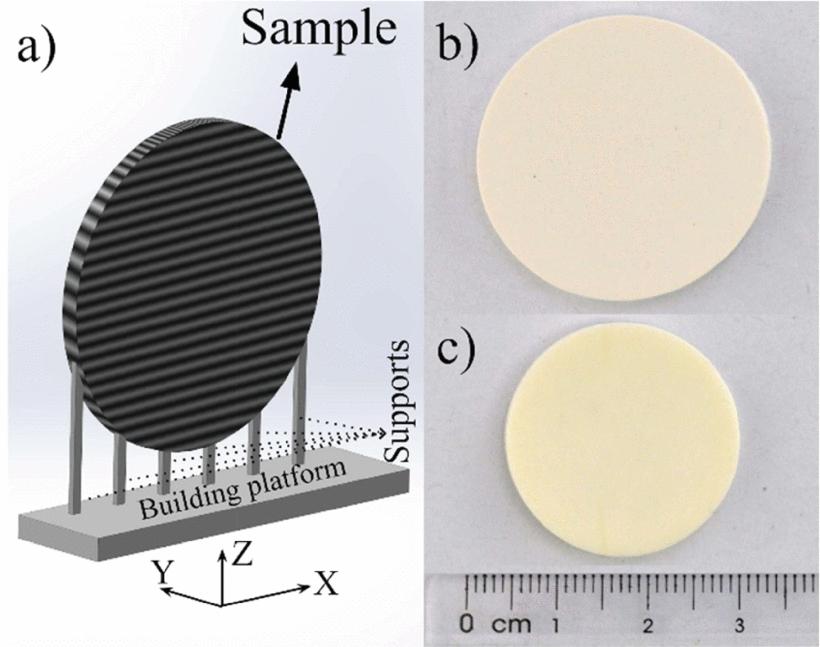
\includegraphics[scale=0.4]{images/5_chapter05/ornik1abc-3047514-large.png}
    \caption{Schematic image of the a) printed sample as well as photographs of b) green and c) sintered Alumina. Source: \cite{Ornik2021}}
    \label{fig:ornik1abc}
\end{figure}

It was further shown that the direction of the slow axis was parallel to the printing direction. A sketch of how the samples are printed is shown to the left in figure \ref{fig:ornik1abc}, where the arrow indicates the printing direction. The top right side shows an actual image of the green sample and the bottom right shows an image of the sample after sintering. For the sintering step the sample is slowly heated to \SI{1700}{\celsius} which causes it to shrink, in this case by around \SI{21}{\volpercent}. In total two different samples were characterized and the result of this characterization is shown in figure \ref{fig:ri_abs} \cite{Ornik2021}. The left plot shows the measured refractive index and the birefringence along the slow and fast direction for the two samples as a function of the frequency, while the right plot shows the measured absorption coefficient for the two samples and directions as a function of the frequency. We see that within the error range the birefringence of the two samples is equal. Therefore, either sample parameters works for setting up the loss function, we use the measurement result from sample 1. 

\begin{figure}[h]
    \centering
    \includestandalone[scale=0.73]{5_chapter05/plots/ceramic/ri_bf}
    \caption{Left plot shows the refractive index and birefringence as a function of frequency for the two ceramic \ce{Al2O3} samples; Sample1 and Sample2. For both samples the refractive index was measured for the perpendicular slow and fast axes. Considering the error margins both samples have an equal birefringence. The right plot shows the absorption coefficient, again for the slow and fast axis of the samples. Data: \cite{Ornik2021}}
    \label{fig:ri_abs}
\end{figure}

Stacking a number of these ceramic discs or plates like the one shown in figure \ref{fig:ornik1abc} we can in theory construct an AWP similar to the TAQ by Masson. This ceramic AWP can then serve as a comparison to the TAQ and therefore also partly as a verification of the loss function at least for the $\lambda/4$ AWP type. In this case the loss functions $L_{\lambda/4}$ and $L_{\lambda/2}$ only depend on the set of angles and thicknesses. In other words the birefringence does not change at each iteration and is the same for each individual plate. Using the thicknesses and angles of the TAQ given in table \ref{tab:masson_result} as well as the birefringence of quartz as reported in \cite{DGrischkowsky1990} we can calculate $L_{\lambda/4}(\nu)$ for the TAQ and use it for comparison. To that end we optimized $L_{\lambda/4}$ for $n=6$ in the range from \SIrange{0.25}{1.50}{\tera \hertz}. The design parameters obtained from this optimization are shown in table \ref{tab:res_cl4} (Result 1). Additionally, the terms of $L_{\lambda/4}(\nu)$ of this result as well as those for the TAQ are plotted in figure \ref{fig:loss_function_cl4} as a function of frequency. We see that the magnitude of $L_{\lambda/4}$ for these two results is similar. This indicates that $L_{\lambda/4}$ is also a suitable measure of the quality of the result similar to $L_{M}$. At around \SI{1.5}{\tera \hertz} there is a clear a cut-off for both results. Defining the bandwidth as the ratio between the upper and lower frequency we get a value of  $5=\frac{\SI{1.5}{\tera \hertz}}{\SI{0.3}{\tera \hertz}}$. 

\begin{table}[h]
    \centering
    \includestandalone{5_chapter05/ceramic_result_table}
    \caption{}
    \label{tab:res_cl4}
\end{table}

\begin{figure}[h]
    \centering
    \includestandalone[scale=1.00]{5_chapter05/plots/ceramic/loss_function}
    \caption{}
    \label{fig:loss_function_cl4}
\end{figure}

Similar to quartz, the birefringence of the ceramic plates is relatively low. This in turn means that for the waveplates to have an effect in the lower end of the spectrum the individual plates must be fairly thick so that we get a total thickness of around \SI{32}{\milli \meter}. Although, if we shift the frequency range of the optimization to \SIrange[range-phrase=-, range-units=single]{0.5}{2.25}{\tera \hertz} then we obtain a second result (result 2) for which the bandwidth is still around $5\approx\frac{\SI{2.25}{\tera \hertz}}{\SI{0.5}{\tera \hertz}}$. With that the total thickness of the AWP can be reduced to \SI{26}{\milli \meter} compared to the \SI{32}{\milli \meter} of result 1. The design parameters of result 2 are given in the lower half of table \ref{tab:res_cl4} and the dotted line in figure \ref{fig:loss_function_cl4} shows the individual terms of $L_{\lambda/4}$ for each frequency bound by the available material data range. 


\begin{itemize}
    \item loss function. Frequency dependent loss.
    \item Circularity. Linearity.
    \item Ellipses. not sure how to plot this yet?
    \item Transmission along two directions.
    \item Retardance, Diattenuation
    \item See what interface does?
    \item Eigenstates?
    \item compare to Result 1 -> we do shorter range because of absorption (thinner plate(s))
    \item high abs compared to quartz (\cite{DGrischkowsky1990})
\end{itemize}

\subsection{Simulation}
\subsection{CST}
\subsection{Fabrication error}

\section{Polymer}

\section{Fused silica glass}

% Todo ref?


